%%%%%%%%%%%%%%%%%%%%%%%%%%%%%%%%%%%%%%%%%
% Thin Sectioned Essay
% LaTeX Template
% Version 1.0 (3/8/13)
%
% This template has been downloaded from:
% http://www.LaTeXTemplates.com
%
% Original Author:
% Nicolas Diaz (nsdiaz@uc.cl) with extensive modifications by:
% Vel (vel@latextemplates.com)
%
% License:
% CC BY-NC-SA 3.0 (http://creativecommons.org/licenses/by-nc-sa/3.0/)
%
%%%%%%%%%%%%%%%%%%%%%%%%%%%%%%%%%%%%%%%%%

%----------------------------------------------------------------------------------------
%	PACKAGES AND OTHER DOCUMENT CONFIGURATIONS
%----------------------------------------------------------------------------------------

\documentclass[a4paper, 11pt]{article} % Font size (can be 10pt, 11pt or 12pt) and paper size (remove a4paper for US letter paper)
\usepackage[ruled]{algorithm2e}
\usepackage[protrusion=true,expansion=true]{microtype} % Better typography
\usepackage{graphicx} % Required for including pictures
\usepackage{wrapfig} % Allows in-line images
\usepackage{amsmath, amsfonts}
\usepackage{hyperref}
\usepackage{subfigure}
\usepackage{booktabs}
\usepackage[numbers]{natbib}
\usepackage[usenames,dvipsnames]{color}
\newcommand{\stnote}[1]{\textcolor{Blue}{\textbf{ST: #1}}}
\newcommand{\menote}[1]{\textcolor{Red}{\textbf{ME: #1}}}

\usepackage{mathpazo} % Use the Palatino font
\usepackage[T1]{fontenc} % Required for accented characters
\linespread{1.05} % Change line spacing here, Palatino benefits from a slight increase by default
\makeatletter
\renewcommand\@biblabel[1]{\textbf{#1.}} % Change the square brackets for each bibliography item from '[1]' to '1.'
\renewcommand{\@listI}{\itemsep=0pt} % Reduce the space between items in the itemize and enumerate environments and the bibliography

\renewcommand{\maketitle}{ % Customize the title - do not edit title and author name here, see the TITLE block below
\begin{flushright} % Right align
{\LARGE\@title} % Increase the font size of the title

\vspace{50pt} % Some vertical space between the title and author name

{\large\@author} % Author name
\\\@date % Date

\vspace{40pt} % Some vertical space between the author block and abstract
\end{flushright}
}

%----------------------------------------------------------------------------------------
%	TITLE
%----------------------------------------------------------------------------------------

\title{\textbf{Incrementally Interpreting Multimodal Referring Expressions in Real Time}} % Subtitle

\author{\textsc{Miles Eldon}\\ % Author
\textsc{Professor Stefanie Tellex} (Reader and Advisor)\\
{\textsc{Professor Michael Littman} (Second Reader)}
\\{\textit{Brown University}}} % Institution

\date{\today} % Date

%----------------------------------------------------------------------------------------

\begin{document}

\maketitle % Print the title section
\newpage
\tableofcontents
\newpage
\section{Introduction}
Robots have long been a great asset in controlled settings, such as factories, yet remain unable to make the crucial leap into daily life, interacting with humans. In order for humans and robots to collaborate in complex tasks, robots must be able to understand people's references to objects in the real world. For example, a robotic assistant might be asked to fetch a tool in a factory setting, or medicine in a hospital setting, or ingredients in a kitchen. Figure~\ref{fig:example} shows Baxter handing a bowl to a chef. To refer to objects, people use a fluid combination of speech, gesture, eye gaze, and a variety of other body language. People provide these referring expressions continiously, and can change rapidly based on new information from the agent they are instructing or their perception of the environment. This new information from a partner can be in the form of confirming signals, such as nodding of the head, or requests for clarification, such as looking confused or asking questions.~\citet{clark96} refers to this back and forth of instruction and clarification or confirmation as a \textit{joint activity}, used to assist in collaborative tasks by creating common ground and reducing uncertainty.


Responding quickly and accurately are critical for a truly interactive robotic assistant in everyday life. By continously interpreting human referring expressions, a robotic assistant can not only respond quickly, but also incorporate the relative timing of gestures and speech in a natural manner. Continous interpretation make interactions more rapid and fluid, and also enable a robot to provide affirming or clarifying feedback in a time frame that is reasonable. This rapid feedback makes these human robot interactions more meaningful by quickly leading to mutual understanding, either with both agents proceeding with their own tasks, or with the human clarifying a request for the robot, rather than necessitating a different system of the human confirming that a request was understood.

\begin{figure}
\centering
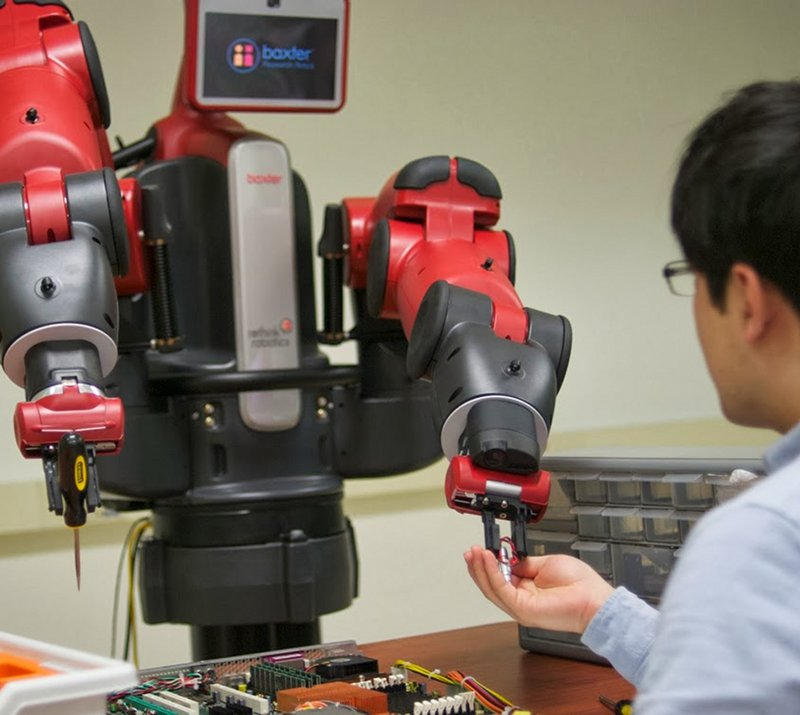
\includegraphics[width=0.3\linewidth]{images/baxter_scene_cropped.jpg}
\caption{Robots that collaborate with people need to understand their
  references to objects in the environment.  For example, if a person
  asks for a tool using language and gesture, the robot needs to
  interpret the person's reference in order to pick up the correct
  tool.\label{fig:example}}
\end{figure}

Despite the importance of a system capable of real-time response to multimodal input, existing models approaches fail to meet this high bar. Several systems focus on single modalities, which are insufficient to handle complicated interactions, such as ambigious phrases accompanied by gestures or vice versa~\citep{tellex11, kollar10}. Approaches that have incorporated multiple sources have failed to do so in an online manner, relying on batch interpretation, which is not fast enough for systems that need to respond immediately~\citep{matuszek14}. These approaches preclude rapid reaction, clarifying feedback, and the level of interpretation necessiated by human referring expressions.

To provide a foundation for these capabilities, we propose a Bayes Filter to interpret information from language and gesture~\citep{thrun08}. Our framework relies on a factored observation probability that fuses information from language and gesture in real time to continuously estimate the object a human user is referencing. We initially demonstrate our model in simulation, and then perform user studies with our system running live to demonstrate its efficacy. The results show that our model quickly and effectively fuses multimodal information in real time to continously estimate the object being referenced. Additionally, we demonstrate a robot that uses our model to provide feedback in the form of facial expressions, pointing, and handing the user the object referenced in real time by interepreting gesture and language.

\begin{figure*}
\centering
\subfigure[Ambiguous gesture.\label{fig:confused}]{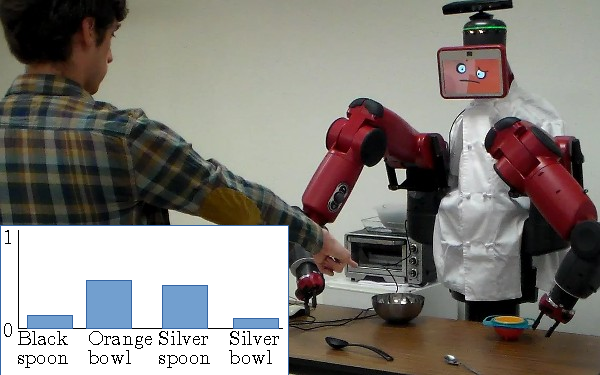
\includegraphics[width=0.49\linewidth]{images/cartoon1.pdf}}
\subfigure[Clarification with language.\label{fig:clarified}]{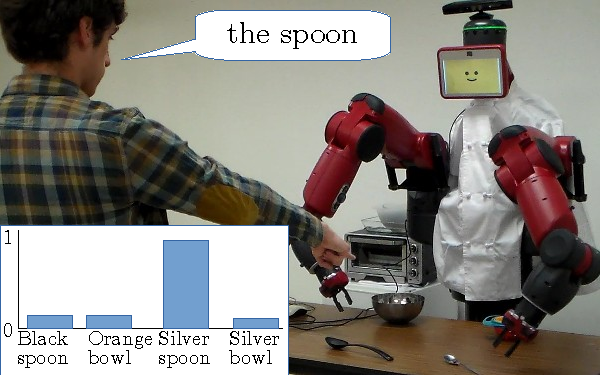
\includegraphics[width=0.49\linewidth]{images/cartoon2.pdf}}
\caption{After an ambiguous gesture, the model has a uniform
  distribution between two objects (a).  The robot responds by
  indicating confusion.  Clarification with language causes a
  probabilistic update leaving the model highly confident it has
  inferred the correct object (b).  The robot responds by smiling and
  pointing to the correct object. \label{fig:cartoon}}
\end{figure*}

\section{Related Work}
~\citep{clark96} proposed that conversation is a \textit{joint activity}, a coordinated, collaboraitve process in which the two participants establish \textit{common ground}. Common ground refers to the process by which each participant establishs an understanding about the beliefs of the other. In order to establish common ground, people use various forms of feedback, ranging from head nods to looks of confusion to explicit clarifying questions. These forms of feedback allows the participants to iteratively establish common ground through instruction and clarification as time progresses. Our Bayes Filter approach provides a foundation for producing this feedback with a robot, which has the ability to increase robustness of human-robot communication through the establishment of common ground during interactions.


\section{Assumptions}
\section{Technical Approach}
\subsection{Transition Model}
\subsection{Observation Model}
\subsubsection{Null Words and Gestures}
\subsubsection{Model Parameters}
\section{Evaluation}
\subsection{Simulation Results}
\subsection{User Studies}
\section{Future Work}
\section{Conclusion}
\end{document}